% プロジェクト学習中間報告書書式テンプレート ver.1.0 (iso-2022-jp)

% 両面印刷する場合は `openany' を削除する
\documentclass[openany,11pt,papersize]{jsbook}

% 報告書提出用スタイルファイル
\usepackage[final]{funpro}%最終報告書
%\usepackage[middle]{funpro}%中間報告書

% 画像ファイル (EPS, EPDF, PNG) を読み込むために
\usepackage[dvipdfmx]{graphicx,color}

% ここから -->
\usepackage{calc,ifthen}
\newcounter{hoge}
\newcommand{\fake}[1]{\whiledo{\thehoge<70}{#1\stepcounter{hoge}}%
  \setcounter{hoge}{0}}
% <-- ここまで 削除してもよい

\usepackage{here}

% 年度の指定
\thisYear{2015}

% プロジェクト名
\jProjectName{フィールドから創る地域・社会のためのスウィフトなアプリ開発}

% [簡易版のプロジェクト名]{正式なプロジェクト名}
% 欧文のプロジェクト名が極端に長い(2行を超える)場合は、短い記述を
% 任意引数として渡す。
%\eProjectName[Making Delicious curry]{How to make delicious curry of Hakodate}
\eProjectName{“Swift” Application Development Based on Field Research}


% <プロジェクト番号>-<グループ名>
\ProjectNumber{3-C}

% グループ名
\jGroupName{教育系グループ}
\eGroupName{Education Group}

% プロジェクトリーダ
\ProjectLeader{1013220}{新保遥平}{Yohei~Shinpo}

% グループリーダ
\GroupLeader  {1013015}{中進吾}{Shingo~Naka}

% メンバー数
\SumOfMembers{5}
% グループメンバ
\GroupMember  {1}{1013130}{熊谷優斗}{Yuto~Kumagai}
\GroupMember  {2}{1013116}{皀勢也}{Seiya~Kurokome}
\GroupMember  {3}{1013220}{新保遥平}{Yohei~Shinpo}
\GroupMember  {4}{1013015}{中進吾}{Shingo~Naka}
\GroupMember  {5}{1013104}{矢吹渓悟}{Keigo~Yabuki}

% 指導教員
\jadvisor{伊藤恵,奥野拓,原田泰,木塚あゆみ,南部美砂子}
% 複数人数いる場合はカンマ(,)で区切る。カンマの前後に空白は入れない。
\eadvisor{Kei~Itou,Taku~Okuno,Yasushi~Harada,Ayumi~Kizuka,Misako~Nanbu}

% 論文提出日
\jdate{2015年7月29日}
\edate{July~29, 2015}

%%%%%%%%%%%%%%%%%%%%%%%%%%%%%%%%%%%%%%%
\usepackage{graphicx}
%%%%%%%%%%%%%%%%%%%%%%%%%%%%%%%%%%%%%%%
\begin{document}
%
% 表紙
\maketitle

%前付け
\frontmatter

% 和文概要
\begin{jabstract} 
%\fake{ここに日本語の概要を書きます。}
 本プロジェクトは教育というフィールドを調査し、教育に関する問題を解決するiOSアプリを開発することを目的としている。

 5月のプロジェクトでは、各メンバーが教育に関わるアプリを考え、メンバーと担当教員にプレゼンテーションを行った。メンバー間では情報の共有を行い、担当教員からはレビューを受けた。その後、担当教員から受けたレビューを基に、お互いにアイデアを広げテーマを1つに絞り込んだ。テーマは、大学生向けプログラミング入門アプリに決まった。

 テーマが決まった後、アプリの設計を行った。しかし、要件定義を固めずにアプリの設計を行ったため、一貫性のないアプリ設計になってしまった。そのため、要件定義を1から考え直すことになった。要件定義を考え直すことは、1度で終わらず何度も行った。その結果、中学校でプログラミングを学んだ人、興味を持った人を対象にしたゲームアプリというテーマに決まった。

 中間発表では、私たちが考えた提案をポスターにまとめ、ポスターセッションを行った。教員や他学生からの評価シートには、「最終的なゴールは?」、「まだ内容が決まっていないので評価不能」、「既存のもとの比較がない」などの意見をいただき、もう1度要件定義を見直しアプリの設計をやり直す必要があることに気付かされた。

 今後は、アプリの設計をやり直しアプリを実装していくことを考えている。また、11月に開催されるアカデミックリンクにてワークショップを開き、そこで得たレビューをもとにアプリを改善していくことを考えている。

% 和文キーワード
%\begin{jkeyword}
%キーワード1, キーワード2, キーワード3, キーワード4, キーワード5
%\end{jkeyword}
\bunseki{中進吾}
\end{jabstract}

%英語の概要
\begin{eabstract} 
%\fake{you should write your English abstract in one page. }
 This project is having for its object to investigate a field as education and develop the iOS application useful for education.

 Each member considered the application of educating and presented a members and teachers on the first of a project. We shared information between the members and received reviews from teachers. After that ideas was expanded each other and the theme was narrowed down to 1 based on the review we received from teachers. The theme was decided in a programming guide application for college students.

 After the theme was decided, the application was designed. But the design of application had inconsistent because the application was designed without making the requirement definition hard. Therefore we changed the requirement definition from one. We didn't finish changing the requirement definition and went many times. As a result, it was decided in a theme as the game application that made the person who learned a programming at junior high school and an interested person the subject.

 The proposition that we thought was gathered in a poster and a poster session was performed in the middle announcement. We received opinions of which "what is last goal", "having no comparison it exists down", " the contents aren't decided yet, so evaluation is impossible" in an evaluation seat from teachers and other students, and the requirement definition was reconsidered again, and they made notice that it's necessary to redo a design of an application.

 We are thinking the design of application is being redone from now on and an application is being mounted. A workshop will be opened in the academic link held in November and we get the review and are thinking an application is being improved. 
% 英文キーワード
%\begin{ekeyword}
%Keyrods1, Keyword2, Keyword3, Keyword4, Keyword5
%\end{ekeyword}
\bunseki{中進吾}
\end{eabstract}

\tableofcontents% 目次


\mainmatter% 本文のはじまり

\chapter{背景}
\section{世界と日本のプログラミング教育について}
現在、世界中でプログラミング教育の必要性が高まっている。政府が公教育としてプログラミングを取り入れている、または取り入れようとしている国が増えてきている[1]。イギリスでは、5歳から16歳の義務教育の新カリキュラムに、プログラミングが正式導入されている[1]。また、エストニアでは小学校1年生から、アプリ開発の授業を開始することになっている[1]。日本でも2012年から中学校の技術家庭科で、プログラミング教育が必修項目となっている[2]。

日本では、ビジュアルプログラミング言語の図1.1のScratchや図1.2のビュートビルダーなどを用いて、ラジコンなどの機械を動かす授業を行っている[3][4]。
\begin{figure}[H]
\begin{center}
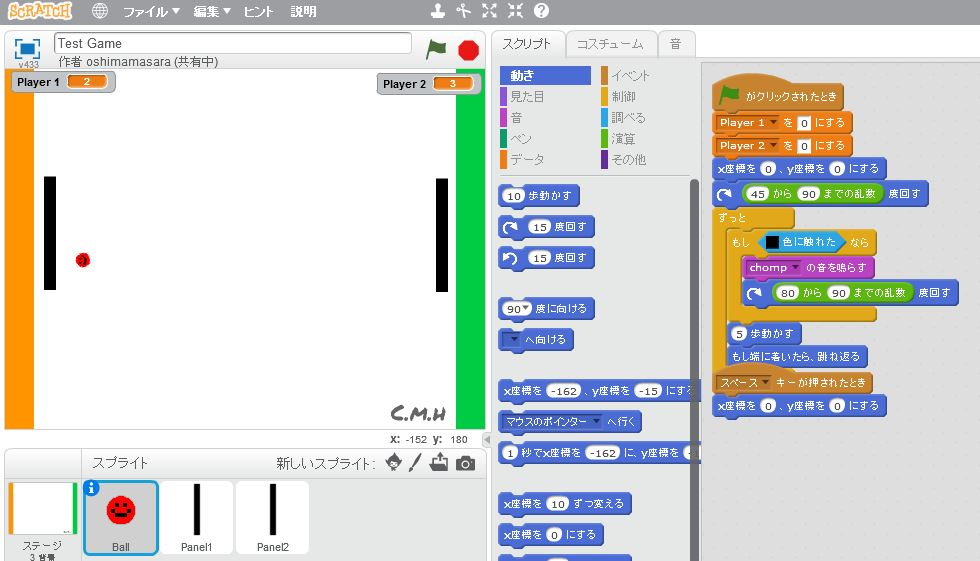
\includegraphics[width=15cm, bb=0 0 1206 950]{img/scratch.jpg}
\end{center}
\caption{Scratchの画面}
\end{figure}



\begin{figure}[H]
\begin{center}
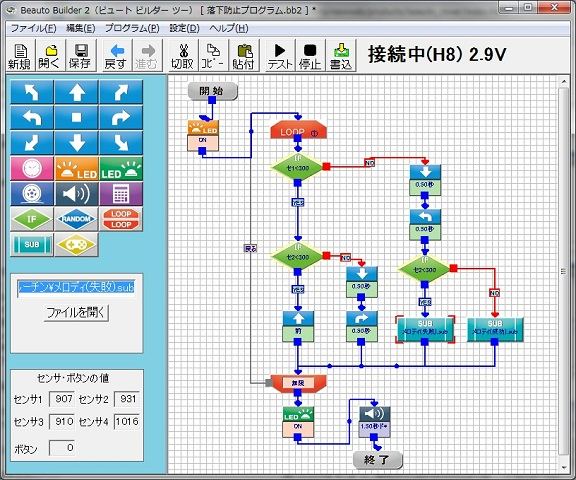
\includegraphics[width=15cm, bb=0 0 1206 1050]{img/Byudo.jpg}
\end{center}
\caption{ビュートビルダーの画面}
\end{figure}
また、2013年6月5日に安倍政権の経済政策「アベノミクス」の「第3の矢」として発表した成長戦略の素案には、「産業競争力の源泉となるハイレベルな IT人材の育成・確保」という項目があった[1]。その中には「義務教育段階からのプログラミング教育等のIT教育を推進する」との記載があった[1]。今後、日本のプログラミング教育はさらに拡大していくことが予想される。

しかし、今の中学校のプログラミング教育ではソースコードを打ってプログラミングをするということを行っておらず、プログラミングの内容を深く取り上げていない。また、プログラミングを学べるのは中学校3年生の時だけで、イギリスやエストニアと比べるととても短い期間である。高校では、実際にプログラミングを教えているところもあるが、義務化さていないので誰もが学校でプログラミングを学べるわけではない[5]。
\bunseki{中進吾}

\section{現状と課題}
日本の中学校ではビジュアルプログラミング言語を用いたプログラミングの授業を行っており、ソースコードを書く練習は行っていない。ビジュアルプログラミング言語はC言語やJavaのようなプログラミング言語と表記の仕方が大きく異なっている。そのため中学校の授業だけでは、C言語やJavaのように実際に文字を打ち込むようなソースコードを組もうとした時、どのように組んでいいかわからない。Webサイトやアプリなどのシステム開発を行う際、基本は文字を打ち込むプログラミング言語を用いるので、ビジュアルプログラミング言語はほとんど使用しない。今の中学校のプログラミング教育だけでは、産業競争力の源泉となるハイレベルな IT人材の育成・確保をすることはできない。現状のままでは、イギリスやエストニアなどの他国との差が広がる一方である。
\bunseki{中進吾}

\chapter{本プロジェクトの目標}
\section{開発アプリの目標}
背景で述べたように、世界中でプログラミング教育の必要性が高まっており、実際に小学生からアプリ開発の授業を行っている国もある。日本でも中学校の技術家庭科でプログラミング教育が必修項目となっている。しかし、現在の中学校のプログラミング教育ではソースコードを打ってプログラミングをするということをしておらず、プログラミングの内容を深く取り上げていない。
\par
そのため、中学校でプログラミングを学んだ人、興味をもった人を対象として、中学で学んだプログラミングと実際のプログラミングの間のプロセスを支援し、ソースコードの組み立てを学ぶことが出来るゲームアプリを開発する。そこで、ビュートビルダーやScratchのようなビジュアルプログラミング言語を学んだ中学生が、C言語のように実際に文字を打ち込むようなソースコードの組み方を理解できるようになることが、開発アプリの目標である。
\bunseki{皀勢也}

\section{プロジェクト学習としての目標}
新しいプログラミング言語であるSwift言語を使い、アジャイル開発手法の一つであるScrumという方法論を用いて素早いアプリ開発をする。また、短期間での開発とフィードバックを繰り返し、より良い品質のアプリ開発を目指している。さらに、バージョン管理システムの理念を学び、効率よくアプリ開発する。プロジェクト学習を通して、情報システムコース、高度ICTコースや情報デザインコースなど異なるコースのメンバーで開発を進めていく。開発を進めていく中で、コミュニケーション能力、グループ開発力を養い、異なる分野の知識を吸収する。
\par
プロジェクト学習としての最終的な目標はアカデミックリンク、成果発表会や課外発表会でアプリの発表を行いレビューを受け、受けたレビューを反映させたアプリをリリースすることである。
\bunseki{皀勢也}

%3章
\chapter{これまでの活動}

\section{プロジェクト全体としての活動}

\subsection{スクラッチワークショップへの参加}
\par 教育をテーマにするに当たり、まず小学生と触れ合い、教育の現状について考えるために、原田先生主催のワークショップに参加した。ワークショップは、2015年5月9日に、函館市青年センターにて行われ、小学校5年生から中学校1年生の子供達計10人が参加した。ワークショップの内容は、ビジュアルプログラミング言語「Scratch」を用いて、動きに反応して音が鳴る不思議楽器を作るというものである。当日、メンバーは小学生の側についてプログラミングのアシスタントをした。
\par ワークショップを通して、気づいた点は次の2点である。
\begin{itemize}
\item 子供達は、一度得た知識はすぐに自分のものにしているようだった。今回のワークショップは、前回のワークショップ参加者から引き続き参加している子供が多いということもあって、メンバーが使い方を教えるまでもなく、自力でプログラミングを行っていた。更に、繰り返し文の使い方を教えたところ、「じゃあさ、ここもこうすればいいんじゃない?」と、子供自ら別の点の修正を行っていた。子供の成長能力の高さに驚いた。
\item 前回から参加している子供に、どうして今回も参加したの?と尋ねたところ、「だって、これ(Scratch)楽しいんだもん」と答えた。子供でもプログラミングに興味を持っていることに驚いた。
\end{itemize}

\par また、ワークショップの最後に、参加者の子供達と、その親に向けた簡単なアンケートを実施した。しかし、プロジェクトとしての方針が決まってない状態で作成したアンケートだったため、内容が建設的なものではなく、得たアンケート結果をその後に生かすことが出来なかった。むしろ、アンケート内容に子供にはわかりづらい表現がある、難しい漢字を使っている、子供用と大人用のアンケート用紙の区別がつかないといった問題を発見できたことが、その後に生かせる学びであったと言える。

\bunseki{熊谷優斗}

\subsection{リスク分析}
\par プロジェクトを進めるにあたって起こりうるリスクをメンバーそれぞれで洗い出し、それぞれのリスクに対して発生確率、被害の内容、対処方法を挙げた。図3.1は洗い出したリスクの一部である。

\par リスクの洗い出しをした時点で既に発生していたのが、「メンバーに連絡がつながらない」というリスクだ。前述のスクラッチワークショップにてアンケートを実施したが、このアンケートを作成する際、メンバーの1人に連絡がつながらず、ワークショップ当日になってそのメンバーにアンケート内容のレビューをしてもらった結果、いくつかの不備があることが発覚した。この不備は、そのメンバーが前日にアンケート内容をレビューできていれば気づけたはずである。今後このようなリスクが発生しないよう、メンバー内で1日1回はSkypeやLINEを確認することを義務づけた。

\begin{figure}[H]
\begin{center}
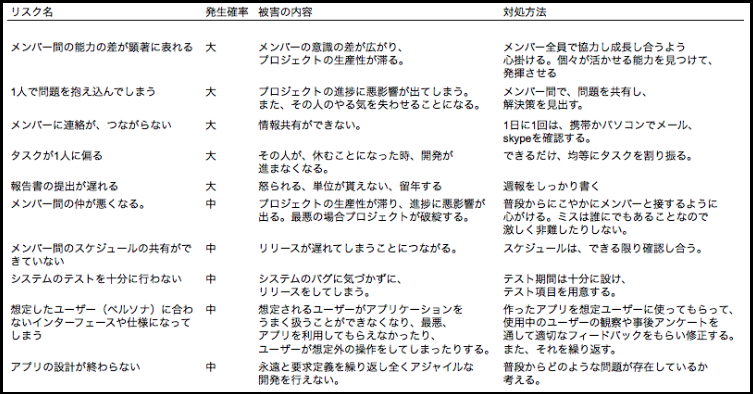
\includegraphics[width=14cm, bb=0 0 753 394]{img/RiskManagement.png}
\end{center}
\caption{リスク分析の結果(一部抜粋)}
\end{figure}

\bunseki{熊谷優斗}

\subsection{アプリ開発のための勉強会}
\par iOSアプリを開発するにあたって必要となる知識を学ぶ勉強会をプロジェクトのティーチングアシスタントが開催したため、これにグループ全員で参加した。勉強会では、XcodeやSwift言語の使い方を学ぶSwift勉強会とバージョン管理システムである、GitとGitHubの使い方を学ぶGitHub勉強会の2種類が行われた。それぞれで行ったことを具体的に記述する。
\par Swift勉強会は全部で3回行われた。第1回では、メンバーそれぞれのPCにXcodeを導入し、Swift言語によってIBLabelやIBButtonを用いた簡単なアプリを作成した。その後、iPadにて作成したアプリをビルドするために、iOS Developer Programへの登録を行った。第2回では、MapKitというFrameworkを用いた地図アプリを作成した。第3回では、サーバーからデータを読み書きすることのできるアプリを作成した。それぞれの回の終わりには演習問題が出され、これを解くことで学んだ知識の復習を行うことができた。
\par GitHub勉強会は全部で3回行われた。それぞれの回を通して、バージョン管理システムの理念を学びつつ、Gitの基本的な使い方を学んでいった。第3回では、Swift勉強の演習問題をGitHubを用いてメンバー間で分担しながら作成せよ、という課題が出た。しかし、上手くコーディングの役割分担を行うことができず、1人で全てのコーディングをし、残りのメンバーでコードレビューをするという形を取った。これに対し、ティーチングアシスタントから昨年度はもっと役割分担ができていた、という報告を受けた。今後、上手く役割分担をしていくために教育班では、GitHub の issue 機能を利用していくことを決定した。
\bunseki{熊谷優斗}

\subsection{バックログの作成}
\par プロジェクトの方針として、アジャイル開発手法の1つであるScrumという方法論を取り入れることが決まっていたため、プロジェクトのスケジュールをバックログを用いて管理した。バックログとは成果物を作り出すために必要な要素を項目に起こした一覧のことで、この一覧を上下に整頓することで項目の優先順位を表す。バックログには明確なスケジューリングをする必要はなく、優先順位の高いものから順番に行っていく。図3.2は6、7月分のバックログの原案である。

\par この原案を企業講師である高森満様と木下実様にお見せしたところ、「バックログの優先度を議論する際にもっと手軽に入れ替えることが可能なように、紙や付箋を用いたほうが良い」というレビューを受けた。そこで、せっかく紙と付箋を使用するならばと、ソフトウェア開発のツールの1つである、「タスクかんばん」のシステムをバックログに取り入れることにした。具体的にはタスクの状態を「TODO」、「DOING」、「DONE」の3つのステージに分割し、更に「TODO」欄のタスクの上下関係によってタスクの優先度を表すようにした。図3.3は実際に使用しているバックログである。

\begin{figure}[H]
\begin{center}
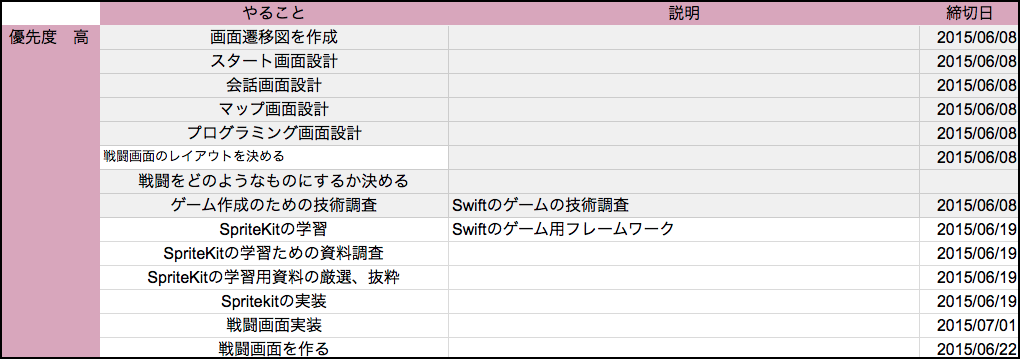
\includegraphics[width=14cm, bb=0 0 1020 359]{img/SprintBacklog.png}
\end{center}
\caption{6、7月分のバックログの原案}
\end{figure}

\begin{figure}[H]
\begin{center}
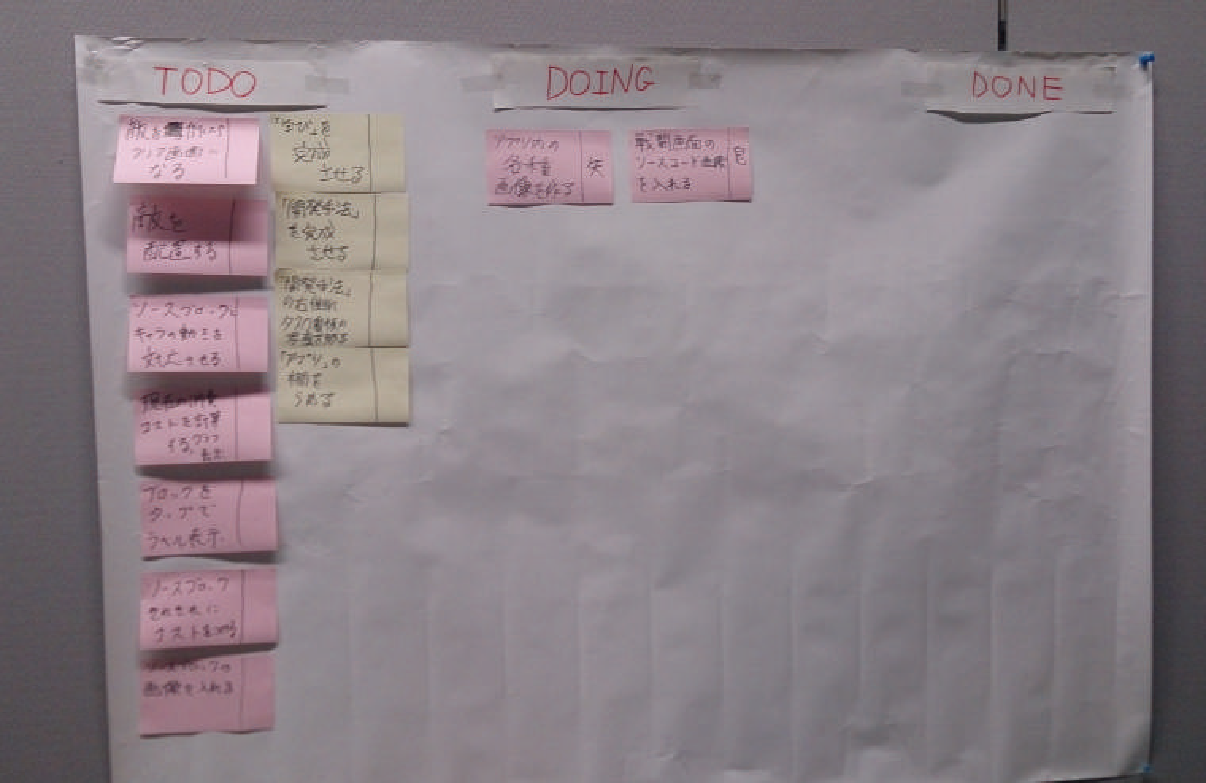
\includegraphics[width=14cm, bb=0 0 1206 783]{img/TaskKanban.png}
\end{center}
\caption{タスクかんばんのシステムを取り入れたバックログ}
\end{figure}

\bunseki{熊谷優斗}

\subsection{中間発表会の資料制作}
\par 中間発表会に向けて、ポスターを制作した。制作にあたって、グループメンバーを実装班3人とポスター班2人に分け、ポスターの制作が終わったら実装班がレビューをする、という形式をとった。しかし、メンバー間の意識共有が上手く行われていなかったため、実装班がポスターのレビューを上手く行うことが出来なかった。そのため、ポスターをティーチングアシスタントや担当教員に見せたところ、目的と制作物がずれている、というレビューを受けた。これを受けて、メンバー5人全員で、一度背景、目的、課題の見直しを行い、ポスターの作り直しをした。しかし、短期間で急いでポスターの作り直しを行ったため、今度は文字が多すぎて見づらいというレビューを受けた。これを受けて、ポスター内の文字を少なくするため、もう一度ポスターの構成を見直すという作業を行った。結果、ポスターを作り上げることができたが、その制作に多くの時間を割くことになってしまった。ポスターやその他ドキュメントを作る際には、まずメンバー間の意識共有を行い、どういった構成で文書を書いていくのかを考えることに時間をかけるべきだ、ということを学んだ。

\bunseki{熊谷優斗}

\subsection{中間発表会}
\par 中間発表会ではメンバーを前半3人、後半2人に分けて、発表を行った。前半の発表では、アプリのデモを行わないと内容が伝わりづらい、というレビューを受けた。これを受けて後半の発表では、デモを取り入れ、内容が伝わりやすいようにした。しかし、後半の発表では合計で9人しか見に来た人がいなかった。このことから、教育系が開発しているアプリに魅力が少ないのではないか、という気づきを得た。

\bunseki{熊谷優斗}

\section{アプリ案の変化と内容}
\par プロジェクトを進めるうちに、アプリ内容、対象ユーザーが変化していった。その内容を以下に記す。
\bunseki{熊谷優斗}

\subsection{アプリ案の検討}
\par メンバーそれぞれが考えて来た案を評価し、5種類の案に絞った。図3.4に案を表す。

\par 5種類それぞれの案をメンバー内で肉付けした後、ティーチングアシスタントと担当教員からレビューを受けた。それぞれの案の詳細とレビューの内容を以下に示す。

\begin{description}
 \item[案1 いじめ対策アプリ]
従来相談を受けてもらうためには、電話をかけ、言葉で喋らなければならないので、ハードルが高い。一部の教育委員会では、メールの対応も行っている。そこで、少しでもハードルを下げるために、LINEのように教育委員会と会話ができるようにする。
\begin{description}
 	\item[レビュー内容]

	このままだとただチャットをするだけのアプリになってしまうのではないか。既存のSNSアプリと差別化を行うため、独自の機能が必要である。また、どのようにしてこのアプリの評価を行うかという点は要検討である。
	 \end{description}
 
  \item[案2 プログラミングを学ぶゲームアプリ]
子供がゲーム攻略を楽しみながら、いつのまにかプログラミングを覚えることができるアプリである。最終的なユーザーの到達点としては制御文が使えるようになることである。
	\begin{description}
 	\item[レビュー内容]
	ゲーム内容は、答えを導くのに手間がかかり、ユーザーに達成感があるものにすべきである。似たようなアプリは既にいくつも存在しているため、それらを調査し、どのように差別化を図るか検討する必要がある。
	 \end{description}

  \item[案3 発想力を鍛える−生産消費的なゲームアプリ]
  ユーザーが生産側と消費側の両面で機能することにより、全ユーザーで一緒に発想力を磨いていくアプリである。自分よがりの発想力ではなく、他人にも共感できる発想力を身につけさせることが目的である。
	\begin{description}
 	\item[レビュー内容]
	ユーザー依存型アプリは投稿が増えないと開発が進まない可能性があるため、どうしたらユーザー同士で活発に活動してもらえるか考えるべきである。
	 \end{description}
	 
 \item[案4 1問1答共有アプリ]
  ユーザーが作った1問1答を共有するアプリである。問題を作る楽しさと問題を解く楽しさをシェアすることができる。
	\begin{description}
 	\item[レビュー内容]
	案3と同様に、どうしたらユーザー同士で活発に活動してもらえるか考える必要がある。投稿者が何か得をするシステムにしなければ問題の投稿数は増えていかないだろう。
	 \end{description}
	 
 \item[案5 外遊び支援アプリ]
遊びの教育を行う。IT化が進み、外で遊ぶことが少なくなってきている子供たちに対し、ITを活用することで子供に外で遊んでもらう機会を増やす。その1つの案として、GPS機能を使って鬼ごっこを行う。
	\begin{description}
 	\item[レビュー内容]
	このアプリを開発するのであれば、楽しく開発を行えるだろう。しかし開発者が楽しくてもユーザーが楽しいとは限らない。ユーザーがどのような遊びを求めているか調査する必要があるだろう。また、アプリを使いながら鬼ごっこをすると、歩きスマホのような状態になり危険なのではないか。
	 \end{description}

 \end{description}
 
 \par レビューを受け、グループ内で検討した結果、前期では「案2 プログラミングを学ぶゲーム」を作成することに決定した。
 
 \begin{figure}[H]
\begin{center}
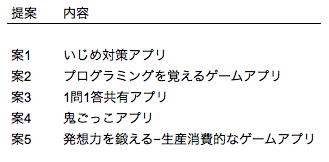
\includegraphics[width=12cm, bb=0 0 329 162]{img/AppIdea.png}
\end{center}
\caption{絞った5種類のアプリ案}
\end{figure}
 
 \bunseki{熊谷優斗}
 
 \subsection{大学生向けプログラミング入門アプリ}
\par 前述の「案2 プログラミングを学ぶゲーム」についてより深く考えていった結果、「既存の類似アプリと相違点を持たせるため、函館要素を追加しよう」、「子供は地域性に対してあまり興味を示さない、ならば対象ユーザーを未来大生にしよう」といった理由から、未来大学に入学することが決まった高校生に対するProcessing導入アプリを作成する方針が決まった。アプリの目的は、未来大1年生が「情報表現入門」でプログラミング言語「Processing」を学ぶ際につまづきやすいポイントを、入学前にゲーム形式で気軽に学んでもらうことである。図3.5と図3.6はアプリ内画面のイメージ図の一部である。

\par 図3.6、通称「プログラミング画面」では、Scratchのように主人公の行動を表すブロックを組み立ててゆく。どのようなブロックを組めばいいかを考え、それにより主人公を操り、敵を全て倒すことがゲームの目的である。更に、「コスト」という概念を定義し、ブロックそれぞれをコストで重み付ける。1ターンで使用できるコストの上限は決まっているので、ユーザーはどのようにブロックを組めば同じコストでも最も多く行動できるかを考える必要がある。例えば、ループ文を使うことで、単純に同じブロックを何度も使用するよりも少ないコストで済む。これによりユーザーは自然と良いアルゴリズムを学ぶことができる。
\par このアプリ案をティーチングアシスタント、担当教員、企業講師の方々に見せたところ、様々なレビューを受けた。一部を抜粋すると次のようなものである。
\begin{itemize}
 \item このアプリをプレイしたところで、本当にプログラミングの教育になるのだろうか。肝心のプログラミング画面の内容が薄く、未来大生がつまづきやすいポイントを学べるとは思えない。どうすればユーザーへの「教育」になるかを練り直すべき。
 \item 大学生が使うにしては、プログラミング画面の内容が低年齢向けである。
 \item もしアプリを一般向けにリリースすることを目標としているのであれば、未来大学入学向けアプリというのは対象ユーザーが狭すぎる。
 \end{itemize}
\par このレビューを受けて、もう一度メンバー内で教育要素について考え直し、対象ユーザーを全国の高校生、大学生向けへと変更した。また、プログラミング画面にて、「→」「パンチ」といった簡単な記述ではなく、「move(right, 3)」「attack(up)」といった、より本物のソースコードに近い形で表示するようにし、そのソースコードはボタンをタップしていくことで組み立てることができる仕組みにした。

\begin{figure}[H]
\begin{center}
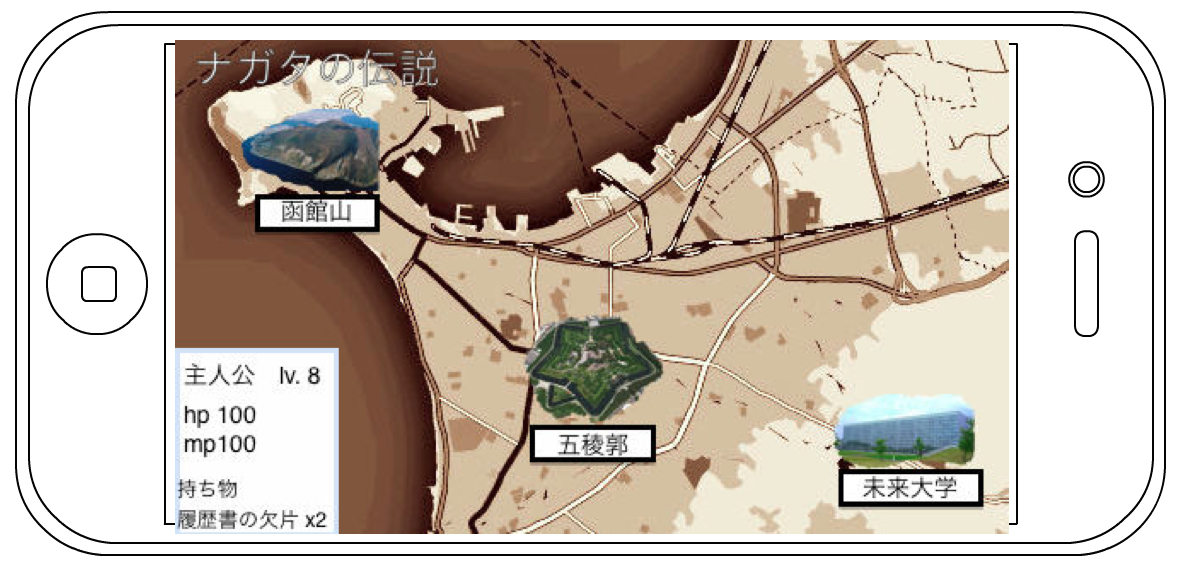
\includegraphics[width=12cm, bb=0 0 1182 571]{img/LengedOfN_map.png}
\end{center}
\caption{マップ画面}
\end{figure}

\begin{figure}[H]
\begin{center}
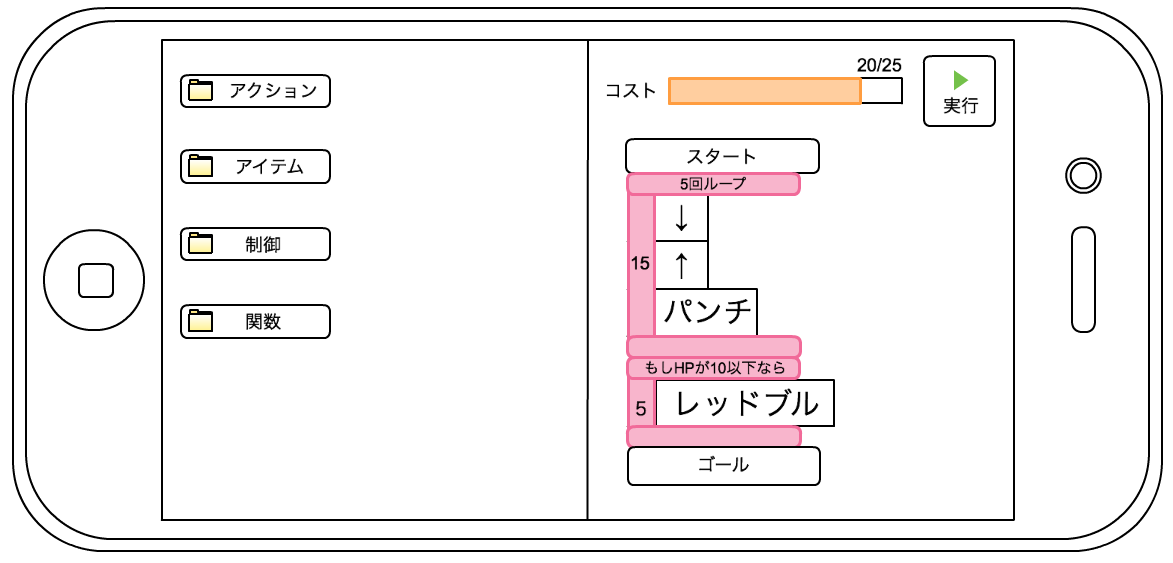
\includegraphics[width=12cm, bb=0 0 1173 563]{img/LegendOfN_programming.png}
\end{center}
\caption{プログラミング画面}
\end{figure}
 \bunseki{熊谷優斗}
 
 \subsection{中学生向けプログラミング支援アプリ}
\par プロジェクトを進めるうちに、大学生向けプログラミング入門アプリでは、プロジェクトとしての背景が、客観的に見て共感されないような内容であることに気がついた。そこで、日本の中学校ではプログラミング教育が義務化されている、また、現状のアプリ内容であれば、小学生、中学生が利用しても問題がないといった理由から、対象ユーザーを変更すべきであるという結論にたどり着いた。この日の議論により生まれたのが現状の背景(第1章にて記載)であり、現状のアプリ案(第4章にて記載)である。

\bunseki{熊谷優斗}

%4章
%%%%%%%%%%%%%%%%%%%%%%%%%%%%%%%%%%%%%%%%%%%%%%%%%%%

\chapter{開発アプリについて}
\section{概要}
開発するアプリは中学生でプログラミングを習った人、興味を持った人を対象としたソースコードの組み方を学ぶゲームアプリである。図4.1のように、このゲームには自機と敵機があり、ユーザーはマス目上のステージにある自機をソースコードを組むことによって動かし、敵機を倒すことでゲームがクリアとなる。

%\\
\begin{itemize}
\item 各ステージのクリアまでの流れ
\end{itemize}
\begin{enumerate}
\item 自機を敵機の前まで移動して倒すソースコードを考える。
\item ソースコードを入力する。
\item ソースコードを実行する。
\item ソースコードの通りに自機が動く。
\item 敵を全て倒すとステージクリアとなる。
\item 使用したコストに合わせてランクとコメントが表示される。
\end{enumerate}
\par 敵機まで移動して倒すまでをいかに短いソースコードで完了させるかを目指すゲームである。

\begin{figure}[h]
\begin{center}
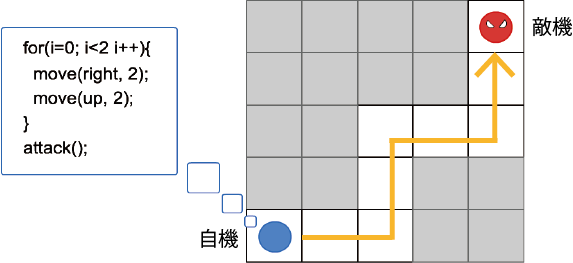
\includegraphics[width=12cm, bb=0 0 573 263]{img/4thParagraph/game.png}
\end{center}
\caption{ゲーム概要}
\end{figure}

\bunseki{新保遥平}

\section{プログラミング画面}
プログラミング画面ではユーザーが敵機を倒すためのソースコードを入力する。例えばfor文を入力したいときは図4.2のように画面に配置されたソースボタンをタップする。

\begin{figure}[H]
\begin{center}
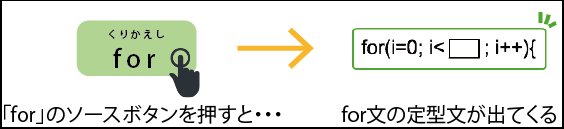
\includegraphics[width=12cm, bb=0 0 564 129]{img/4thParagraph/forButton.png}
\end{center}
\caption{ソースコードの入力}
\end{figure}
ユーザーは図4.3のように画面右側に配置されたそれぞれのソースボタンをタップして、ソースコードを組み立てていく。現状、実装したソースボタンはattack()、move()、left、right、0〜9、;  などである。タップされたソースボタンは順に、右側のスペースに記述される。


\begin{figure}[H]
\begin{center}
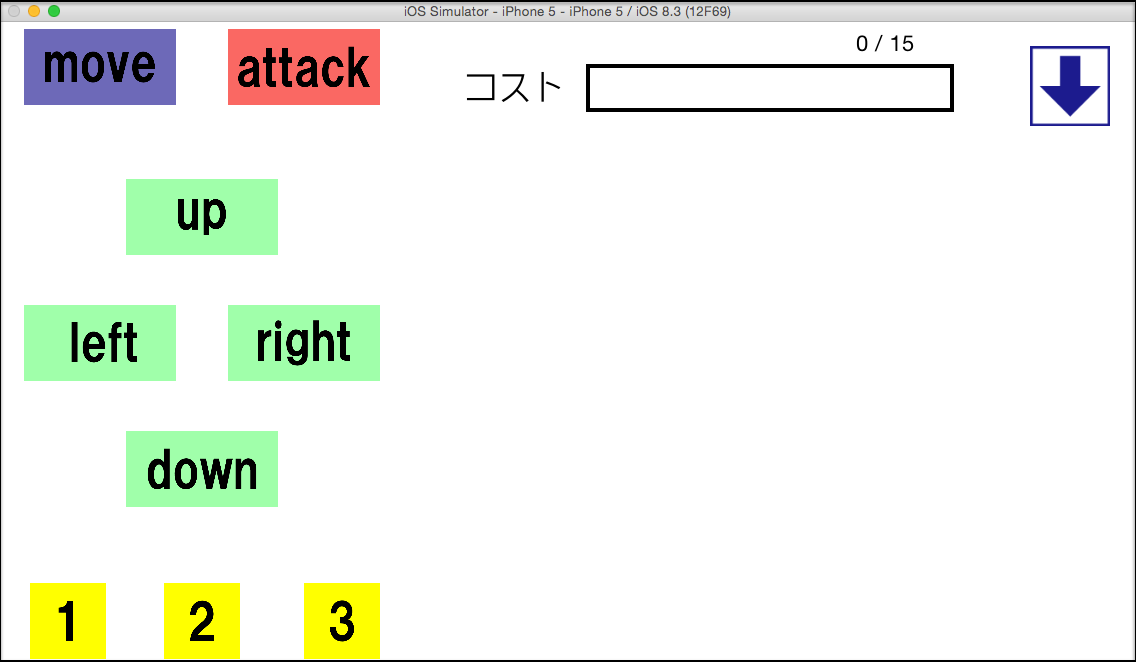
\includegraphics[width=12cm, bb=0 0 1136 662]{img/4thParagraph/Prog-ra_programming.png}
\end{center}
\caption{プログラミング画面}
\end{figure}

例えば下記のようなプログラムを組むこととする。
\par move(right,3);
\par move(up,3);
\\
\\
このソースコードを図4.4のプログラミング画面に入力した。

\begin{figure}[H]
\begin{center}
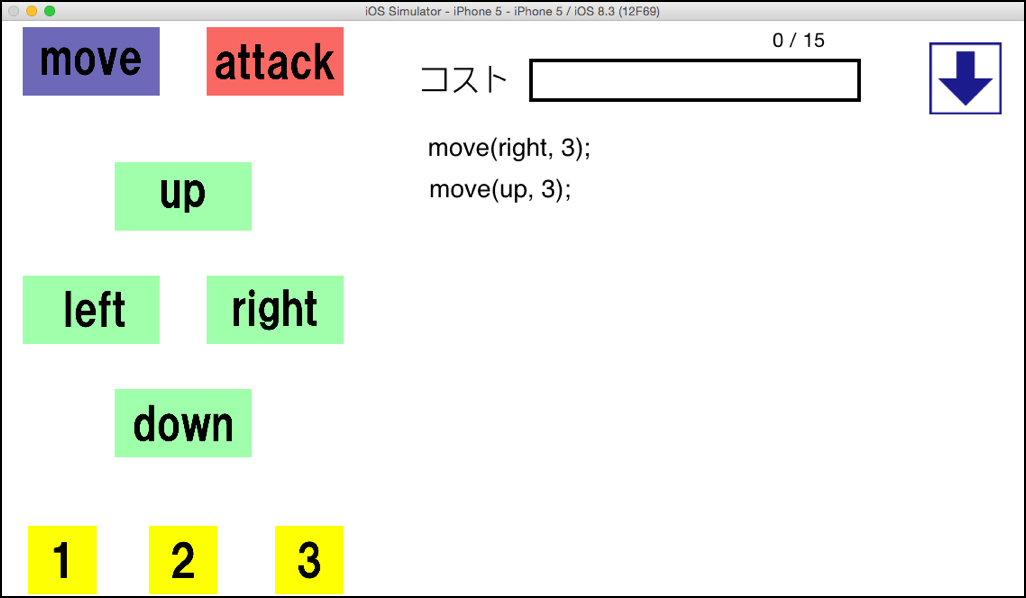
\includegraphics[width=12cm, bb=0 0 1136 662]{img/4thParagraph/Prog-ra_programming1.png}
\end{center}
\caption{ソースコード入力後のプログラミング画面}
\end{figure}

このようにプログラムをタップで組むことが出来る。また、図4.5のようのに、次に引数である数字を入れるべきところに「up」をタップしてしまうなど、間違ったタイミングでソースボタンを押すと画面上にエラーが出て、すぐに確認ができる。


\begin{figure}[H]
\begin{center}
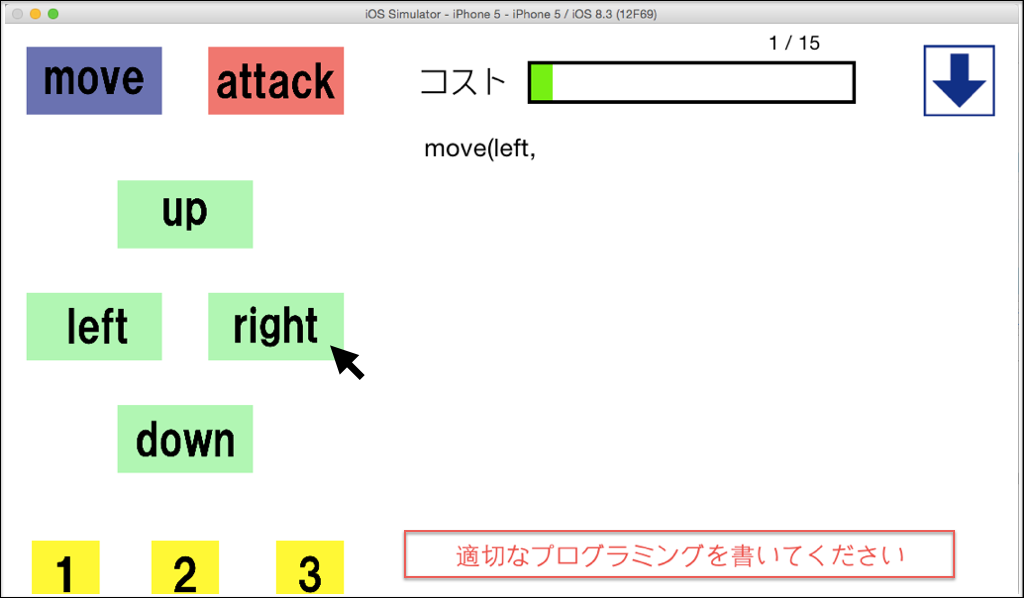
\includegraphics[width=12cm, bb=0 0 1024 598]{img/4thParagraph/error.png}
\end{center}
\caption{ソースコードがエラー時のプログラミング画面}
\end{figure}
ユーザーはソースコードを入力後、プログラミング画面の左上の「下矢印」ボタンで戦闘画面に移動する。

\bunseki{新保遥平}

\section{戦闘画面}
図4.6の戦闘画面はプログラミング画面で入力したソースコードで自機を動かすための画面である。戦闘画面の左下にある三角の実行ボタンを押すことで、自機を動かすことが出来る。また戦闘画面、左下の「P」と書かれたボタンでプログラミング画面に戻ることができる。現状では、あらかじめ設定されたプログラムでしか自機を動かすことが出来ない。

\begin{figure}[H]
\begin{center}
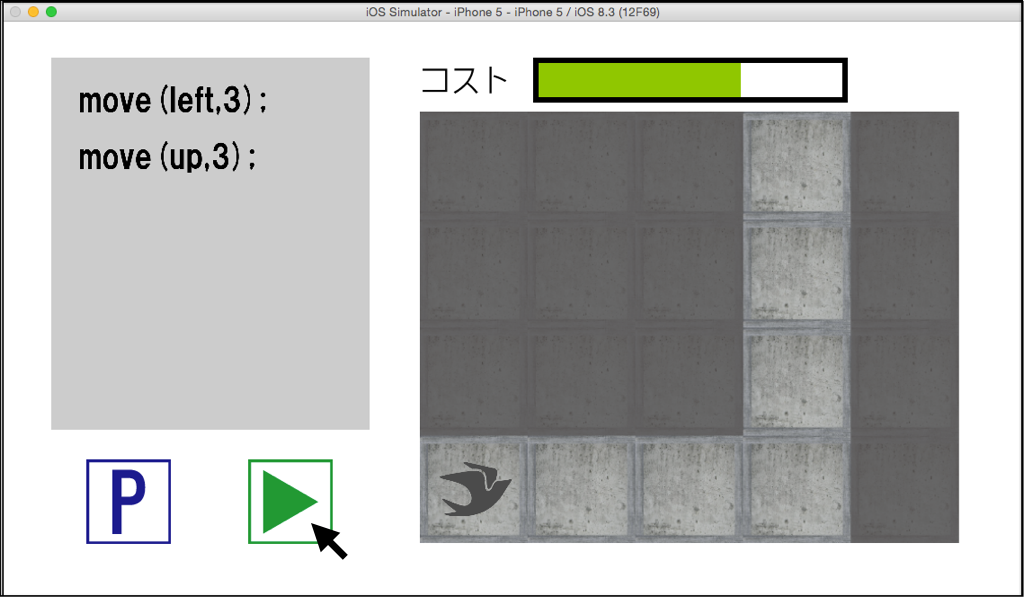
\includegraphics[width=12cm, bb=0 0 1136 662]{img/4thParagraph/Prog-ra_Battle.png}
\end{center}
\caption{戦闘画面}
\end{figure}

\bunseki{新保遥平}

\subsection{ゲーム性}
ただプログラミングを学ぶのではなく、ゲームを通してプログラミングを学ぶことでユーザーのモチベーションを保ちつつ、アプリを使ってもらえると考えた。また実際にソースコードを組むことで自機を思い通りに動かすことが出来たときにプログラミングの学習が深まると考えた。
 
\bunseki{新保遥平}


\subsection{教育性}
このアプリではユーザーがより簡潔なソースコードを組み立てられるようになるために、コストとランクがある。ソースのボタンそれぞれにコストが設けられており、問題をクリアした際にコストの使用量が少ないほど簡潔にソースコードを組み立てることが出来たと判定し、図4.7のようにランクを与える。ランクが低かった場合、より良いランクにつながるヒントを与える。そして高いランクが与えられたときに、ユーザーを褒める言葉を表示する。このサイクルが次の問題への意欲につながり、より簡潔なソースコードを組み立てることが出来るようになる。この流れをユーザーストーリーとしたものを図4.8に示す。

\begin{figure}[H]
\begin{center}
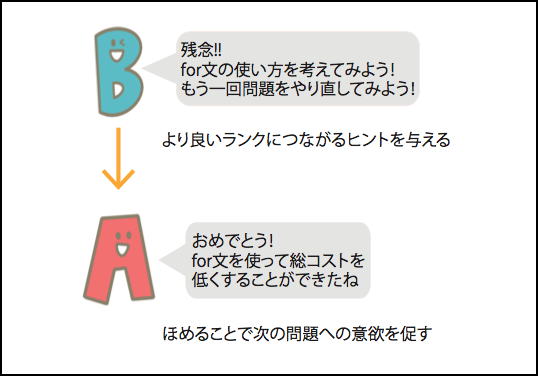
\includegraphics[width=12cm, bb=0 0 538 376]{img/4thParagraph/cost.png}
\end{center}
\caption{ランクとヒント}
\end{figure}

\begin{figure}[H]
\begin{center}
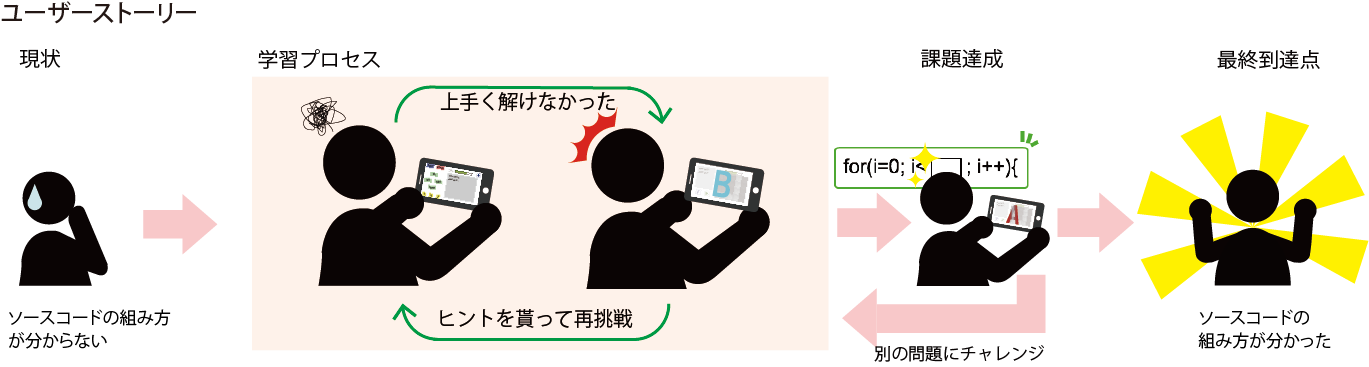
\includegraphics[width=14.5cm, bb=0 0 564 129]{img/4thParagraph/userstory.png}
\end{center}
\caption{ユーザーストーリー}
\end{figure}







\bunseki{新保遥平}
%%%%%%%%%%%%%%%%%%%%%%%%%%%%%%%%%%%%%%%%%%%%%%%%%%%

%5章
\chapter{結果}
\section{プロジェクトの評価}
本プロジェクトは、多くの人からレビューを受け、今の背景、課題、目的になっている。しかし、私たちが考えたアプリはその背景、課題、目的につながっていない。そのため、このプロジェクトは具体的な方針が定まっていない状態である。

また、7月に行われた中間発表会の評価シートの結果からは、「声がはっきり聞こえた」、「声は大きく聞きやすかった」、「相手の顔を見て話してくれたので、聞き取りやすかった」などの意見をいただき、発表技術に関しては高い評価を得られた。しかし、発表内容に関しては「最終的なゴールは?」、「内容がわからないないので評価不能」、「既存のもとの比較がない」などの意見をいただいた。いただいた意見をまとめると、本プロジェクトは目標が決まっておらず、内容がわかりづらいという評価であった。

これらのことから、本プロジェクトは第三者の方に伝えられる内容になっていないので背景、課題、目的につながるアプリ案が必要である。そして、第三者の方に伝えられる内容にしていかなければならない。
\bunseki{中進吾}

\section{プロジェクトの成果}
\par 前期の活動の成果は以下の3点である。
\begin{itemize}
\item スクラッチワークショップに参加したことにより、プログラミング初心者の方にプログラミングを教える場合、C言語やJavaから始めるのではなく、Scratchのようなビジュアルプログラミング言語から始めた方が良いということがわかった。また、プログラミングで音声機器などの機械を動かしてもらうことにより、プログラミングに興味を持ってもらうことができるということがわかった。
\item 
本プロジェクトでは、Swift言語を用いてアプリ実装を行うことになっていた。しかし、メンバー全員Swift言語は使ったことがなかったため、実装に不安があった。アプリを実装できる期間は短かったが、キャラクターを動かしたり、ボタンをタップすることでソースコードを打ち込めることができるところまでアプリを開発することができた。これによって、今後のアプリの実装に対する不安がほとんどなくなった。また、アプリの実装を行えたことにより、実装に携わったメンバーはSwift言語に自信を持つことができた。

\item 中間発表会で展示するポスターは、Adobe Illustratorという描画ツールソフトを使用して作成することになっていた。このソフトを使用したことがあるのはメンバーの5人中2人だけだったため、ポスターを作成できるのは2人だけだった。しかし、3.1.5で述べたように目的と制作物がずれていたため、メンバー 5人全員で、一度 背景、目的、課題の見直しを行い、ポスターを作り直すことになった。その結果、今までAdobe Illustratorを使ったことがない人も使えるようになり、メンバー全員がポスターを作成できるようになった。11月に開催されるアカデミックリンクや最終成果発表でもポスターを使用するので、メンバー全員がポスターを作成できるようになったことは、非常に大きな成果である。
\end{itemize}


\bunseki{中進吾}


\chapter{今後の課題と展望}
\section{アプリ案の課題と展望}
中間発表会で得られたレビューをまとめると、現状のアプリ案は、目標がしっかりと定まっておらず、内容がわかりにくい。今後は、現在のアプリ案を再考し、より具体的で背景、課題、目的が一貫性のあるアプリ案にしていく必要がある。そこで現状のアプリ案を細かく修正していくのか、それとも、また1からアプリ案を考え直し、要件定義をやり直すかは、これからグループで話し合って決めるべき課題である。
\par
話し合いで決めたアプリ案を教育アプリとして体裁を整え、11月に開催されるアカデミックリンクまでに実際に動かすことが出来るプロトタイプを完成させる。アカデミックリンクでワークショップを開き、参加者からプロトタイプのレビューを受け、そこで得たレビューを活かしてアプリの改善を行うことが今後の展望である。
\bunseki{皀勢也}

\section{メンバーの課題と展望}
中間発表会に向けて、プロトタイプを制作する実装班と、ポスターを制作するポスター班で分かれたが、いくつか課題があった。アプリやポスターに使われる画像の制作は情報デザインコースのメンバーがほとんど一人で作っていたため、実装がスムーズにいかなかった。なるべくタスクをメンバーで分散させるべきであった。また、ポスター班は実装に関わっていなかったため、実装班とのスキルの差がある。後期からは全員で実装を行っていくため、ポスター班はSwift言語とバージョン管理システムに慣れていく必要がある。
\par
さらに、プロジェクト学習の授業外での作業が多く、メンバー全員が作業できない日があった。そのため、情報共有に時間がかかったり、効率良く作業をすることができなかった。
\par
今後の展望は、後期からはメンバー全員で実装し、スムーズにアプリ開発を行えるように、タスクを分散させてプロジェクトを進めていき、グループ全体の作業は授業時間内に終わらせることである。また、経験したことない作業でも積極的に取り組み、1人のメンバーにタスクが集中しないように協力していくことである。

\bunseki{皀勢也}

\chapter{学び}
\section{グループとしての学び}
アプリ案の要件定義を固めずに実装を行ったため、対象ユーザや目的が合っていないことが分かった。また、教育系グループとして教育という意味をしっかり決めていなかったため、プロジェクトの目的を見失い要件定義を一から考え直すことになった。そのため、時間をかけて要件定義を行うことの重要性を学んだ。また、プロジェクト学習の授業外での作業が多く、議事録を残していないことがあり、情報共有がうまくできていなかった。このことからドキュメントを残して、情報共有することの大切さを学んだ。
\par
グループでの活動を通してグループメンバーの得意分野、不得意分野を把握し、各メンバーがそれぞれの得意分野を活かせる作業を行うことができた。また、話し合いを重ねることでスムーズに進めることができ、メンバーの適切な役割分担を学んだ。
\bunseki{皀勢也}

\section{各メンバーの学び}
\subsection{熊谷優斗}
\par これまで大学での活動の中で何度かPBLは経験したものの、自ら課題を考え主体的に活動したことは初めての経験だったため、様々な学びを得ることができた。その中でも、今回は1つの学びをとりあげる。その学びは、メンバーに技術を教えることの難しさだ。過去のPBL経験から、Gitに関しての知識は持っていたため、メンバーにGitとGitHubの使い方を教える役目を受け持った。しかし、メンバーによって理解度の差があるにも関わらず、理解できているメンバーに合わせて話を進めていってしまった。そのため、メンバー全員にGitの使い方を理解してもらうことができなかった。このことから、メンバーの理解状況を確認し、全員が理解した上で次のステップに進む、という教え方が大切であることを学んだ。
\bunseki{熊谷優斗}

\subsection{皀勢也}
本プロジェクトを進めるにあたって、Swift言語を使ってプログラミングを行うため、Xcodeが入っているMacOSが必要であった。自分はWindowsのノートパソコンしか持っていなかったため、enPiTからMacBook Airを借りて作業を行った。初めは、Windowsと異なり上手く作業を進めれなかったが、使っているうちにMacOSに慣れて上手く作業できるようになった。
\par
また、グループで開発を行っていくうちに、他者にもわかりやすいソースコードを書くように意識した。さらに、GitとGitHubを使ってバージョン管理することや議事録を残すことの重要性を学んだ。

\bunseki{皀勢也}

\subsection{新保遥平}
\par 技術的な点ではGitHubをちゃんと理解して使えるようになった。グループ内でもGitHubを上手く使ってアプリの開発や報告書の作成を行った。
\par プロジェクトリーダーとして、人に仕事を振リ分けることの大切さを学んだ。自分一人で行うべきでない仕事も一人で行ってしまったため、自分の仕事の進捗が遅れることがあった。後期からは人それぞれにあった仕事を上手く振り分けられるようにしたい。また、後期からはプロジェクトメンバー全員に分かる見通しの取れたスケジュールを立て、プロジェクトを進ませたい。

\bunseki{新保遥平}

\subsection{中進吾}
\par 仕事を均等に振り分けることができていなかったため、進捗が遅れることがあった。グループリーダーとして後期は、できるだけ仕事が偏らないように心掛け、プロジェクトをまとめていきたい。
\par また、私はこれまでに2度PBLに参加してきたが要件定義は先輩に任して、自分は実装ばかりをやっていた。今回、一から要件定義を考えたことは大きな学びであり、自分に足りないものを見つけることができた。今後、PBLに参加するときには自分から率先して要件定義を立て、この経験を後輩に伝えていきたい。
\bunseki{中進吾}

\subsection{矢吹渓悟}
デザインプロセスの大切さを再認識し、同時に自分の未熟さを痛感した。なぜなら、初期テーマの設定からブレインストーミングやフィールドの調査を怠ってしまったからだ。本来ならば、メンバーが一丸となって、話し合いや現状を調べながら、みんなでテーマを確立するべきだ。しかしながら、今回は個人個人がやりたいものを考え、そこから一つに絞ってしまったのだ。そのため、背景情報や対象ユーザーの設定が偏見や想像論になったり、後付けとなり、プロジェクトの根幹が揺らいでしまい、最終的にテーマの見直しまでに落ちてしまった。よって、今後テーマを見直す上で大切なのは、ブレインストーミングなどを通していろいろな可能性を吟味した上で、徐々に一つに絞り込むことが大切だと再認識した。
\bunseki{矢吹渓悟}

% 以降、付録(付属資料)であることを示す
\begin{appendix}

\chapter{新規習得技術}
%\begin{hissu}
%課題解決過程に習得した技術について解説する。
%\end{hissu}

\chapter{活用した講義}
%\begin{hissu}
%課題解決過程において活用した講義について、講義名・活用内容を記述する。 
%\end{hissu}

\chapter{相互評価}
%\begin{hissu}
%課題解決過程で分担し、連携した作業全般について、互いに客観的に評価する。 
%\end{hissu}

\chapter{その他製作物}
%\begin{hissu}
%その他成果物をプロジェクトの担当教員の指示に従って添付する。
%\end{hissu}

%付録の終わり
\end{appendix}


%\backmatter

% 参考文献
\begin{thebibliography}{9}
% \bibitem {ラベル} 著者名. 書籍名. 出版社,  年号.
% \bibitem {A2} ほげほげお. うんたらかんたら,  2003.
 \bibitem {A2} Code部. 5歳からプログラミング必修化!?世界の最新IT教育トレンドまとめ |Code部,  2015. \url{http://blog.codecamp.jp/programming_education/} (2015/7/20)
 \bibitem {A2} TechAcademy. プログラミングが義務教育に!政府の成長戦略素案に盛り込まれたプログラミング教育の内容とは |TechAcademyマガジン,  2013. \url{http://techacademy.jp/magazine/736} (2015/7/20)
 \bibitem {A2} 日本経済新聞. 中学の技術・家庭科で「ビジュアルプログラミング」を導入:日本経済新聞,  2012. \url{http://www.nikkei.com/article/DGXNASFK2701H_X21C12A2000000/} (2015/7/20)
 \bibitem {A2} ヴィストン株式会社. 計測器プログラマー |ヴィストン株式会社,  2012. \url{http://www.vstone.co.jp/products/mcprogrammer/} (2015/7/20)
  \bibitem {A2} コードアカデミー高等学校. コードアカデミー高等学校,  2015. \url{http://www.code.ac.jp/} (2015/7/20)
\end{thebibliography}

\end{document}